
%-------------------------------------------------------------------------------
% Pie chart - color
%-------------------------------------------------------------------------------
\begin{figure}
\centering
\def\angle{0}
\def\radius{3}
\def\cyclelist{{"orange","blue","red","green"}}
\newcount\cyclecount \cyclecount=-1
\newcount\ind \ind=-1
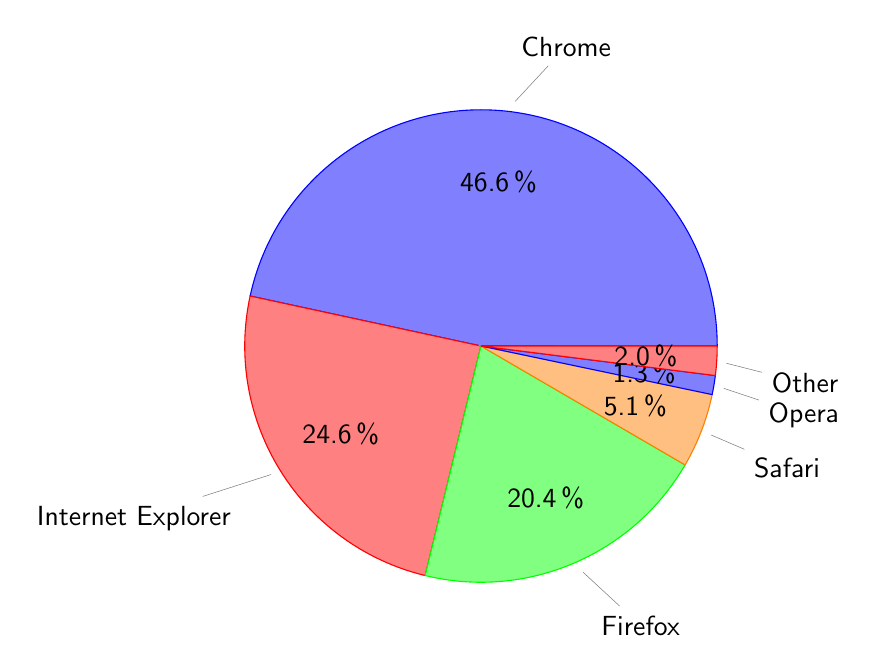
\begin{tikzpicture}[nodes = {font=\sffamily}]
  \foreach \percent/\name in {
      46.6/Chrome,
      24.6/Internet Explorer,
      20.4/Firefox,
      5.1/Safari,
      1.3/Opera,
      2.0/Other
    } {
      \ifx\percent\empty\else               % If \percent is empty, do nothing
        \global\advance\cyclecount by 1     % Advance cyclecount
        \global\advance\ind by 1            % Advance list index
        \ifnum3<\cyclecount                 % If cyclecount is larger than list
          \global\cyclecount=0              %   reset cyclecount and
          \global\ind=0                     %   reset list index
        \fi
        \pgfmathparse{\cyclelist[\the\ind]} % Get color from cycle list
        \edef\color{\pgfmathresult}         %   and store as \color
        % Draw angle and set labels
        \draw[fill={\color!50},draw={\color}] (0,0) -- (\angle:\radius)
          arc (\angle:\angle+\percent*3.6:\radius) -- cycle;
        \node at (\angle+0.5*\percent*3.6:0.7*\radius) {\percent\,\%};
        \node[pin=\angle+0.5*\percent*3.6:\name]
          at (\angle+0.5*\percent*3.6:\radius) {};
        \pgfmathparse{\angle+\percent*3.6}  % Advance angle
        \xdef\angle{\pgfmathresult}         %   and store in \angle
      \fi
    };
\end{tikzpicture}
\caption{Pie chart}
\end{figure}

%-------------------------------------------------------------------------------
% Circular arrows with text
%-------------------------------------------------------------------------------
\begin{figure}
\centering

\begin{tikzpicture}
  \fill[even odd rule,yellow!30] circle (3.8) circle (3.2);
%  \foreach \x in {0,60,...,300} {
%    \arcarrow{3}{3.5}{4}{\x+20}{\x+100}{5}{red,
%      draw = red!50!black, very thick}{napisr \x}
%  }
	
	\arcarrow{3}{3.5}{4}{0}{80}{5}{yellow,
      draw = red!50!black, very thick}{Generacja danych}
    \arcarrow{3}{3.5}{4}{90}{140}{5}{yellow,
      draw = red!50!black, very thick}{Transmisja}
    \arcarrow{3}{3.5}{4}{150}{220}{5}{yellow,
      draw = red!50!black, very thick}{CSA VHDL blok}
    \arcarrow{3}{3.5}{4}{230}{300}{5}{yellow,
      draw = red!50!black, very thick}{CSA Aplikacja}
    \arcarrow{3}{3.5}{4}{310}{360}{5}{green,
      draw = red!50!black, very thick}{Weryfikacja}
\end{tikzpicture}
\caption{Circular arrows with text}
\end{figure}
%-------------------------------------------------------------------------------

%-------------------------------------------------------------------------------
% Inertial navigation system
%-------------------------------------------------------------------------------
% We need layers to draw the block diagram
\pgfdeclarelayer{background}
\pgfdeclarelayer{foreground}
\pgfsetlayers{background,main,foreground}

% Define a few styles and constants
\tikzstyle{sensor}=[draw, fill=blue!20, text width=5em, 
    text centered, minimum height=2.5em]
\tikzstyle{ann} = [above, text width=5em]
\tikzstyle{naveqs} = [sensor, text width=6em, fill=red!20, 
    minimum height=12em, rounded corners]
\def\blockdist{2.3}
\def\edgedist{2.5}

\begin{figure}
\centering
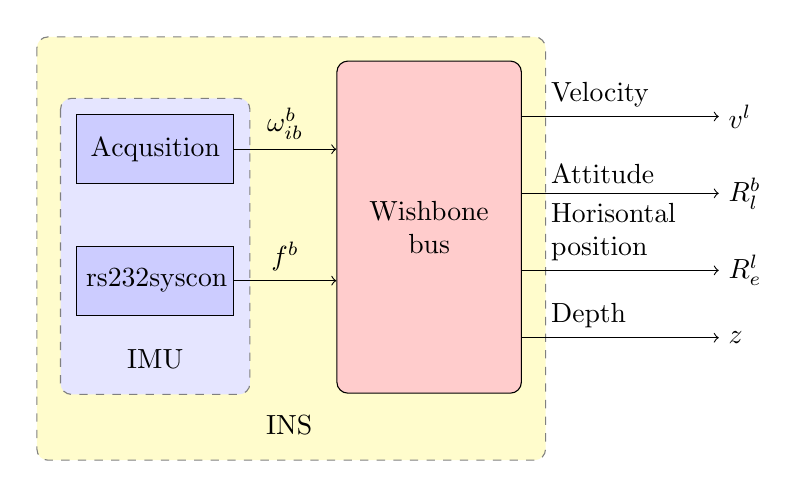
\begin{tikzpicture}
    \node (naveq) [naveqs] {Wishbone \\ bus};
    % Note the use of \path instead of \node at ... below. 
    \path (naveq.140)+(-\blockdist,0) node (gyros) [sensor] {Acqusition};
    \path (naveq.-150)+(-\blockdist,0) node (accel) [sensor] {rs232syscon};
    
    % Unfortunately we cant use the convenient \path (fromnode) -- (tonode) 
    % syntax here. This is because TikZ draws the path from the node centers
    % and clip the path at the node boundaries. We want horizontal lines, but
    % the sensor and naveq blocks aren't aligned horizontally. Instead we use
    % the line intersection syntax |- to calculate the correct coordinate
    \path [draw, ->] (gyros) -- node [above] {$\vc{\omega}_{ib}^b$} 
        (naveq.west |- gyros) ;
    % We could simply have written (gyros) .. (naveq.140). However, it's
    % best to avoid hard coding coordinates
    \path [draw, ->] (accel) -- node [above] {$\vc{f}^b$} 
        (naveq.west |- accel);
    \node (IMU) [below of=accel] {IMU};
    \path (naveq.south west)+(-0.6,-0.4) node (INS) {INS};
    \draw [->] (naveq.50) -- node [ann] {Velocity } + (\edgedist,0) 
        node[right] {$\vc{v}^l$};
    \draw [->] (naveq.20) -- node [ann] {Attitude} + (\edgedist,0) 
        node[right] { $\mx{R}_l^b$};
    \draw [->] (naveq.-25) -- node [ann] {Horisontal position} + (\edgedist,0)
        node [right] {$\mx{R}_e^l$};
    \draw [->] (naveq.-50) -- node [ann] {Depth} + (\edgedist,0) 
        node[right] {$z$};
    
    % Now it's time to draw the colored IMU and INS rectangles.
    % To draw them behind the blocks we use pgf layers. This way we  
    % can use the above block coordinates to place the backgrounds   
    \begin{pgfonlayer}{background}
        % Compute a few helper coordinates
        \path (gyros.west |- naveq.north)+(-0.5,0.3) node (a) {};
        \path (INS.south -| naveq.east)+(+0.3,-0.2) node (b) {};
        \path[fill=yellow!20,rounded corners, draw=black!50, dashed]
            (a) rectangle (b);
        \path (gyros.north west)+(-0.2,0.2) node (a) {};
        \path (IMU.south -| gyros.east)+(+0.2,-0.2) node (b) {};
        \path[fill=blue!10,rounded corners, draw=black!50, dashed]
            (a) rectangle (b);
    \end{pgfonlayer}
\end{tikzpicture}
\caption{Circular arrows with text}
\end{figure}

%-------------------------------------------------------------------------------

%-------------------------------------------------------------------------------
% State machine
%-------------------------------------------------------------------------------
\begin{figure}
\centering
\begin{tikzpicture}[->,>=stealth',shorten >=1pt,auto,node distance=2.8cm,
                    semithick]
  \tikzstyle{every state}=[fill=red,draw=none,text=white]

  \node[initial,state] (A)                    {$q_a$};
  \node[state]         (B) [above right of=A] {$q_b$};
  \node[state]         (D) [below right of=A] {$q_d$};
  \node[state]         (C) [below right of=B] {$q_c$};
  \node[state]         (E) [below of=D]       {$q_e$};

  \path (A) edge              node {0,1,L} (B)
            edge              node {1,1,R} (C)
        (B) edge [loop above] node {1,1,L} (B)
            edge              node {0,1,L} (C)
        (C) edge              node {0,1,L} (D)
            edge [bend left]  node {1,0,R} (E)
        (D) edge [loop below] node {1,1,R} (D)
            edge              node {0,1,R} (A)
        (E) edge [bend left]  node {1,0,R} (A);
\end{tikzpicture}
\caption{State machine}
\end{figure}
%-------------------------------------------------------------------------------

%-------------------------------------------------------------------------------
% Computer science mindmap
%-------------------------------------------------------------------------------

\begin{figure}
\centering
\begin{tikzpicture}
  \path[mindmap,concept color=black,text=white]
    node[concept] {Computer Science}
    [clockwise from=0]
    child[concept color=green!50!black] {
      node[concept] {practical}
      [clockwise from=90]
      child { node[concept] {algorithms} }
      child { node[concept] {data structures} }
      child { node[concept] {pro\-gramming languages} }
      child { node[concept] {software engineer\-ing} }
    }  
    child[concept color=blue] {
      node[concept] {applied}
      [clockwise from=-30]
      child { node[concept] {databases} }
      child { node[concept] {WWW} }
    }
    child[concept color=red] { node[concept] {technical} }
    child[concept color=orange] { node[concept] {theoretical} };
\end{tikzpicture}
\caption{State machine}
\end{figure}
%-------------------------------------------------------------------------------

\begin{figure}[hbt!]
\centering
\begin{tikzpicture}[node distance=1cm, auto,]
 %nodes
 \node[punkt] (market) {Generacja danych testowych};
 \node[punkt, inner sep=5pt,below=0.5cm of market]
 (formidler) {Weryfikacja danych};
 % We make a dummy figure to make everything look nice.
 \node[above=of market] (dummy) {};
 \node[right=of dummy] (t) {CSA VHDL blok}
   edge[pil,bend left=45] (market.east) % edges are used to connect two nodes
   edge[pil, bend left=45] (formidler.east); % .east since we want
    ;                                         % consistent style
 \node[left=of dummy] (g) {CSA Aplikacja}
   edge[pil, bend right=45] (market.west)
   edge[pil, bend right=45] (formidler.west)
   edge[pil,<->, bend left=45] node[auto] {transmisja} (t);
\end{tikzpicture}
\caption{Schemat scenariusza testowego.}
\label{fig:circ_arrow}
\end{figure}